%%%%%%%%%%%%%%%%%%%%%%%%%%%%%%%%%%%%
%% Template file SP 2024
%% Include in directory homework.sty and headerfooter.tex
%%%%%%%%%%%%%%%%%%%%%%%%%%%%%%%%%%%%

\documentclass[12pt]{article}
\usepackage{homework}

\graphicspath{{images/}}
\geometry{letterpaper, portrait, includeheadfoot=true, hmargin=1in, vmargin=1in}

\setcounter{section}{-1}
%% Solution hiding %%
\usepackage[utf8]{inputenc}
\usepackage{lipsum}


\begin{document}
\singlespacing

\renewcommand{\familydefault}{\rmdefault}
\pagestyle{fancy}
\fancyhf{}
\setlength{\headheight}{30pt}
\renewcommand{\headrulewidth}{0.4pt}
\renewcommand{\footrulewidth}{0.4pt}
\lhead{\large Homework 2 \\ Due Feb. 20, 2024 }
\rhead{\large CS 446 \\ Spring 2024}
\rfoot{\textbf{Page \thepage}}
\lfoot{}

\section{Instructions}

Homework is due Tuesday, April 16, 2024 at 23:59pm Central Time.
Please refer to \url{https://courses.grainger.illinois.edu/cs446/sp2024/homework/hw/index.html} for course policy on homeworks and submission instructions.

\section{GAN: 5pts}
\begin{enumerate}
    \item The problem will be:
    \[\max_{\mathcal{D}}\mathbb{E}_{x \sim p_r(x)}[\log\mathcal{D}(x)] + \mathbb{E}_{x \sim p_g(x)}[\log(1-\mathcal{D}(x))] \]
    which is equivalent to maximize:
    \[\int p_r(x)\log\mathcal{D}(x)+ p_g(x)\log(1-\mathcal{D}(x))\,dx\]
    Hence, the optimal choice of $\mathcal{D}(x)$ is:
    \[\mathcal{D}^*(x) = \frac{p_r(x)}{p_r(x) + p_g(x)}\]

    \item Plugged in the optimal $\mathcal{D}(x)$, Eq. 1 will turn into:
    \[\min_{\mathcal{G}}\mathbb{E}_{x \sim p_r(x)}\left[\log\frac{p_r(x)}{p_r(x) + p_g(x)}\right] + \mathbb{E}_{x \sim p_g(x)}\left[\log\frac{p_g(x)}{p_r(x) + p_g(x)}\right]\]
    which is equivalent to minimize:
    \[\int p_r(x)\log\frac{p_r(x)}{p_r(x) + p_g(x)}\,dx + \int p_g(x)\log\frac{p_g(x)}{p_r(x) + p_g(x)}\,dx\]
    \[= D_{\text{KL}}(p_r(x)\|p_r(x)+p_g(x)) + D_{\text{KL}}(p_g(x)\|p_r(x)+p_g(x))\]
    \[= 2D_{\text{JS}}(p_r(x);p_g(x))\]
    Therefore, when $\mathcal{D}$ reaches optimal, optimizing Eq. 1 is the same as minimizing $D_{\text{JS}}(p_r(x);p_g(x))$.

    \item When $\mathcal{D}$ perfectly classifies generated samples, the output of $\mathcal{D}$ will saturate and the gradient of $\mathcal{D}$ will be almost 0, which makes the gradient of $\mathcal{G}$ almost 0 as well.
\end{enumerate}
\newpage

\section{Diffusion model: 11pts}
\begin{enumerate}
    \item \[\text{ELBO}_{\theta}(\textbf{\textit{x}}_0) = \sum_{t=1}^{T}\frac{1}{2\sigma^2}\frac{\beta_{t}(1-\overline{\beta}_{t-1})}{\overline{\beta}_{t}^{2}}\mathbb{E}_{q(\textbf{\textit{x}}_t|\textbf{\textit{x}}_0)}\left[\|\hat{\textbf{\textit{x}}}_{\theta}(\textbf{\textit{x}}_t)-\textbf{\textit{x}}_0\|_2^2\right]\]
    
    where $\overline{\beta}_t := 1 - \prod_{i=1}^{t}(1-\beta_i)$.
    \item No, because $p_{\theta}(\cdot)$ represent the reconstruction process from random noise in diffusion models and thus cannot directly give the likelihood of an existing test sample.
    
    \item \[q(\textbf{\textit{x}}_t|\textbf{\textit{x}}_0) = \prod_{i=1}^{t}q(\textbf{\textit{x}}_i|\textbf{\textit{x}}_{i-1}) = \prod_{i=1}^{t}\mathcal{N}(\textbf{\textit{x}}_i;\sqrt{1-\beta_i}\textbf{\textit{x}}_{i-1},\beta_i\textbf{I})\]
    \[\textbf{\textit{x}}_t = \sqrt{1 - \beta_t}\textbf{\textit{x}}_{t-1} + \sqrt{\beta_t}\bm{\epsilon}_{t-1} = \sqrt{1 - \beta_t}\sqrt{1 - \beta_{t-1}}\textbf{\textit{x}}_{t-2} + \sqrt{\beta_t}\bm{\epsilon}_{t-1} + \sqrt{1 - \beta_t}\sqrt{\beta_{t-1}}\bm{\epsilon}_{t-2}\]
    We can estimate covariance of the new Gaussian noise $\sqrt{\beta_t}\bm{\epsilon}_{t-1} + \sqrt{1 - \beta_t}\sqrt{\beta_{t-1}}\bm{\epsilon}_{t-2}$:
    \[\bm{\sigma}_{t-2} = [(\sqrt{\beta_t})^2 + (\sqrt{1 - \beta_t}\sqrt{\beta_{t-1}})^2]\mathbf{I} = [\beta_t + \beta_{t-1} - \beta_t\beta_{t-1}]\mathbf{I} = [1-(1-\beta_t)(1-\beta_{t-1})]\mathbf{I}\]
    and thus:
    \[\textbf{\textit{x}}_t = \sqrt{(1-\beta_t)(1-\beta_{t-1})}\textbf{\textit{x}}_{t-2} + \sqrt{1 - (1-\beta_t)(1-\beta_{t-1})}\bm{\epsilon}_{t-2}\]
    \[= \sqrt{(1-\beta_t)(1-\beta_{t-1})(1-\beta_{t-2})}\textbf{\textit{x}}_{t-3} + \sqrt{1 - (1-\beta_t)(1-\beta_{t-1})(1-\beta_{t-2})}\bm{\epsilon}_{t-3}\]
    \[=\dots=\sqrt{\prod_{i=1}^{t}(1-\beta_i)}\textbf{\textit{x}}_0 + \sqrt{1-\prod_{i=1}^{t}(1-\beta_i)}\bm{\epsilon}_0\]
    \[= \sqrt{1-\overline{\beta}_t}\textbf{\textit{x}}_0 + \sqrt{\overline{\beta}_t}\bm{\epsilon}_0\]
    where $\overline{\beta}_t := 1 - \prod_{i=1}^{t}(1-\beta_i)$. Hence, as $\textbf{\textit{x}}_t\sim q(\textbf{\textit{x}}_t|\textbf{\textit{x}}_0)$, we have:
    \[q(\textbf{\textit{x}}_t|\textbf{\textit{x}}_0) = \mathcal{N}(\textbf{\textit{x}}_t | \sqrt{1-\overline{\beta}_t}\textbf{\textit{x}}_0,\,\overline{\beta}_t\mathbf{I})\]
    \[\overline{\beta}_t := 1 - \prod_{i=1}^{t}(1-\beta_i)\]
    \newpage

    \item From the last question we can get:
    \[q(\textbf{\textit{x}}_t|\textbf{\textit{x}}_{t-1},\textbf{\textit{x}}_0)\frac{q(\textbf{\textit{x}}_{t-1}|\textbf{\textit{x}}_0)}{q(\textbf{\textit{x}}_t|\textbf{\textit{x}}_0)} = \mathcal{N}(\textbf{\textit{x}}_t | \sqrt{1-\beta_t}\textbf{\textit{x}}_{t-1},\,\beta_t\mathbf{I})\frac{\mathcal{N}(\textbf{\textit{x}}_{t-1} | \sqrt{1-\overline{\beta}_{t-1}}\textbf{\textit{x}}_0,\,\overline{\beta}_{t-1}\mathbf{I})}{\mathcal{N}(\textbf{\textit{x}}_t | \sqrt{1-\overline{\beta}_t}\textbf{\textit{x}}_0,\,\overline{\beta}_t\mathbf{I})}\]
    \[\propto\exp\left(\frac{(\textbf{\textit{x}}_t - \sqrt{1-\beta_t}\textbf{\textit{x}}_{t-1})^2}{2\beta_t} + \frac{\left(\textbf{\textit{x}}_{t-1} - \sqrt{1-\overline{\beta}_{t-1}}\textbf{\textit{x}}_0\right)^2}{2\overline{\beta}_{t-1}} - \frac{\left(\textbf{\textit{x}}_{t} - \sqrt{1-\overline{\beta}_{t}}\textbf{\textit{x}}_0\right)^2}{2\overline{\beta}_{t}}\right)\]
    Denote the polynomial in the above exponential as $r(\textbf{\textit{x}}_{t-1}, \textbf{\textit{x}}_t, \textbf{\textit{x}}_0)$. Since $q(\textbf{\textit{x}}_{t-1}|\textbf{\textit{x}}_t,\textbf{\textit{x}}_0)$ is a Gaussian distribution, minimize $r$ with respect to $\textbf{\textit{x}}_{t-1}$ should lead to the mean $\mu_\theta(\textbf{\textit{x}}_t,\textbf{\textit{x}}_0)$. Hence, taking derivative of $r$ with respect to $\textbf{\textit{x}}_{t-1}$:
    \[\frac{\partial r}{\partial \textbf{\textit{x}}_{t-1}} = \frac{-\sqrt{1-\beta_t}\textbf{\textit{x}}_t + (1-\beta_t)\textbf{\textit{x}}_{t-1}}{\beta_t} + \frac{-\sqrt{1-\overline{\beta}_{t-1}}\textbf{\textit{x}}_{0} + \textbf{\textit{x}}_{t-1}}{\overline{\beta}_{t-1}} = 0\]
    \[\Rightarrow \frac{\beta_t+\overline{\beta}_{t-1}-\beta_t\overline{\beta}_{t-1}}{\beta_t\overline{\beta}_{t-1}}\textbf{\textit{x}}_{t-1} = \left(\frac{\sqrt{1-\beta_t}\textbf{\textit{x}}_t}{\beta_t} + \frac{\sqrt{1-\overline{\beta}_{t-1}}\textbf{\textit{x}}_0}{\overline{\beta}_{t-1}}\right)\]
    \[\Rightarrow \mu_\theta(\textbf{\textit{x}}_t,\textbf{\textit{x}}_0) = \textbf{\textit{x}}_{t-1} = \frac{\overline{\beta}_{t-1}\sqrt{1-\beta_t}\textbf{\textit{x}}_t + \beta_t\sqrt{1-\overline{\beta}_{t-1}}\textbf{\textit{x}}_0}{\beta_t+\overline{\beta}_{t-1}-\beta_t\overline{\beta}_{t-1}}\]
    \newpage

    \item According to Bayes' rule, 
    \[\log p_\theta(\textbf{\textit{x}},\delta|\textbf{\textit{x}}_\text{known}) = \log\frac{p(\textbf{\textit{x}}_\text{known}|\textbf{\textit{x}})p_\theta(\textbf{\textit{x}},\delta)}{p(\textbf{\textit{x}}_\text{known})}\] 
    \[= \log p(\textbf{\textit{x}}_\text{known}|\textbf{\textit{x}}) + \log p_\theta(\textbf{\textit{x}},\delta) - \log p(\textbf{\textit{x}}_\text{known})\]
    Hence we have:
    \[\nabla_\textbf{\textit{x}}\log p_\theta(\textbf{\textit{x}}|\textbf{\textit{x}}_\text{known}) = \nabla_\textbf{\textit{x}}\log p(\textbf{\textit{x}}_\text{known}|\textbf{\textit{x}}) + \nabla_\textbf{\textit{x}}\log p_\theta(\textbf{\textit{x}},\delta) - \nabla_\textbf{\textit{x}}\log p(\textbf{\textit{x}}_\text{known})\]
    \[= \nabla_\textbf{\textit{x}}\log p(\textbf{\textit{x}}_\text{known}|\textbf{\textit{x}}) + \nabla_\textbf{\textit{x}}\log p_\theta(\textbf{\textit{x}},\delta)\]
    Since $p(\textbf{\textit{x}}_\text{known}|\textbf{\textit{x}})\propto\exp(-\|(\textbf{\textit{x}}-\textbf{\textit{x}}_\text{known})\odot\textbf{\textit{M}}\|^2_2)$:
    \[s_\theta(\textbf{\textit{x}},\delta|\textbf{\textit{x}}_\text{known}) = \nabla_\textbf{\textit{x}}\log p_\theta(\textbf{\textit{x}}|\textbf{\textit{x}}_\text{known}) = \nabla_\textbf{\textit{x}}(-\|(\textbf{\textit{x}}-\textbf{\textit{x}}_\text{known})\odot\textbf{\textit{M}}\|_2^2) + \nabla_\textbf{\textit{x}}\log p_\theta(\textbf{\textit{x}},\delta)\]
    \[= s_\theta(\textbf{\textit{x}},\delta) - \nabla_\textbf{\textit{x}}\|(\textbf{\textit{x}}-\textbf{\textit{x}}_\text{known})\odot\textbf{\textit{M}}\|_2^2\]
    \[= s_\theta(\textbf{\textit{x}},\delta) - 2(\textbf{\textit{x}} - \textbf{\textit{x}}_\text{known})\odot\textbf{\textit{M}}\]
\end{enumerate}
\newpage

\section{Unsupervised learning / contrastive learning: 4 pts}
\begin{enumerate}
    \item True.
    \item False. MAE is an approach for computer vision, and the mask-out rate can vary greatly.
    \item True.
    \item False. CLIP does enable zero-shot classification with contrastive pre-training.
\end{enumerate}
\newpage

\section{Coding: GAN, 10pts}
\begin{figure}[!ht]
    \centering
    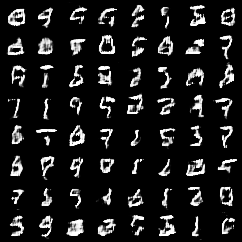
\includegraphics{test_30}
    \caption{Tests after 30 epochs}
\end{figure}
\begin{figure}[!ht]
    \centering
    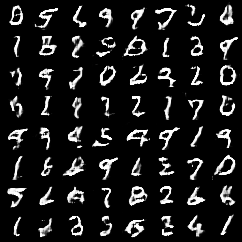
\includegraphics{test_60}
    \caption{Tests after 60 epochs}
\end{figure}
\begin{figure}[!ht]
    \centering
    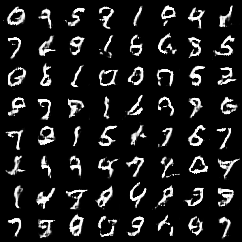
\includegraphics{test_90}
    \caption{Tests after 90 epochs}
\end{figure}
\newpage

\section{Coding: Diffusion model, 10pts}
\begin{enumerate}
    \item[(a)] Visualization of the score function:
    \begin{figure}[!h]
        \centering
        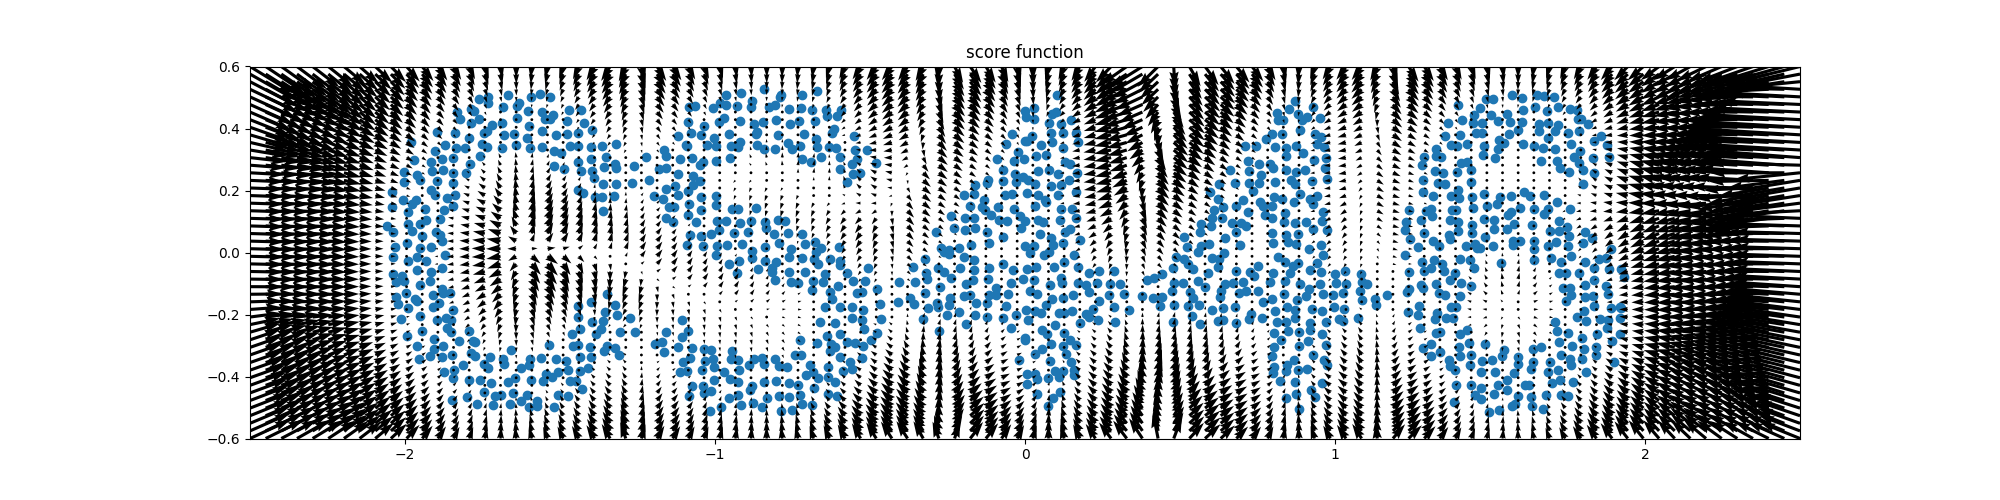
\includegraphics[width=\linewidth]{score}
    \end{figure}
    \item[(b)] Six plots in total (Figure 4 to 9):
    \begin{figure}[!h]
        \centering
        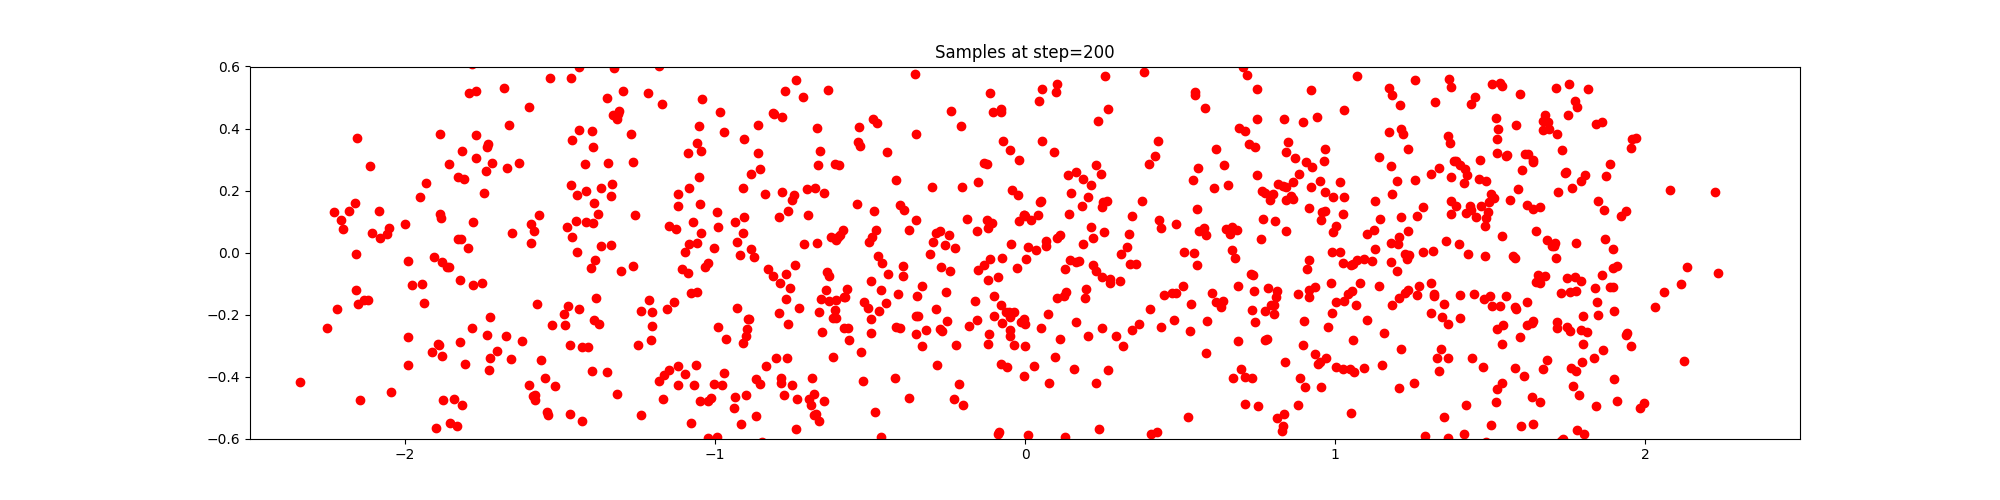
\includegraphics[width=\linewidth]{step_200}
        \caption{Points at time step 200}
    \end{figure}
    \begin{figure}[!h]
        \centering
        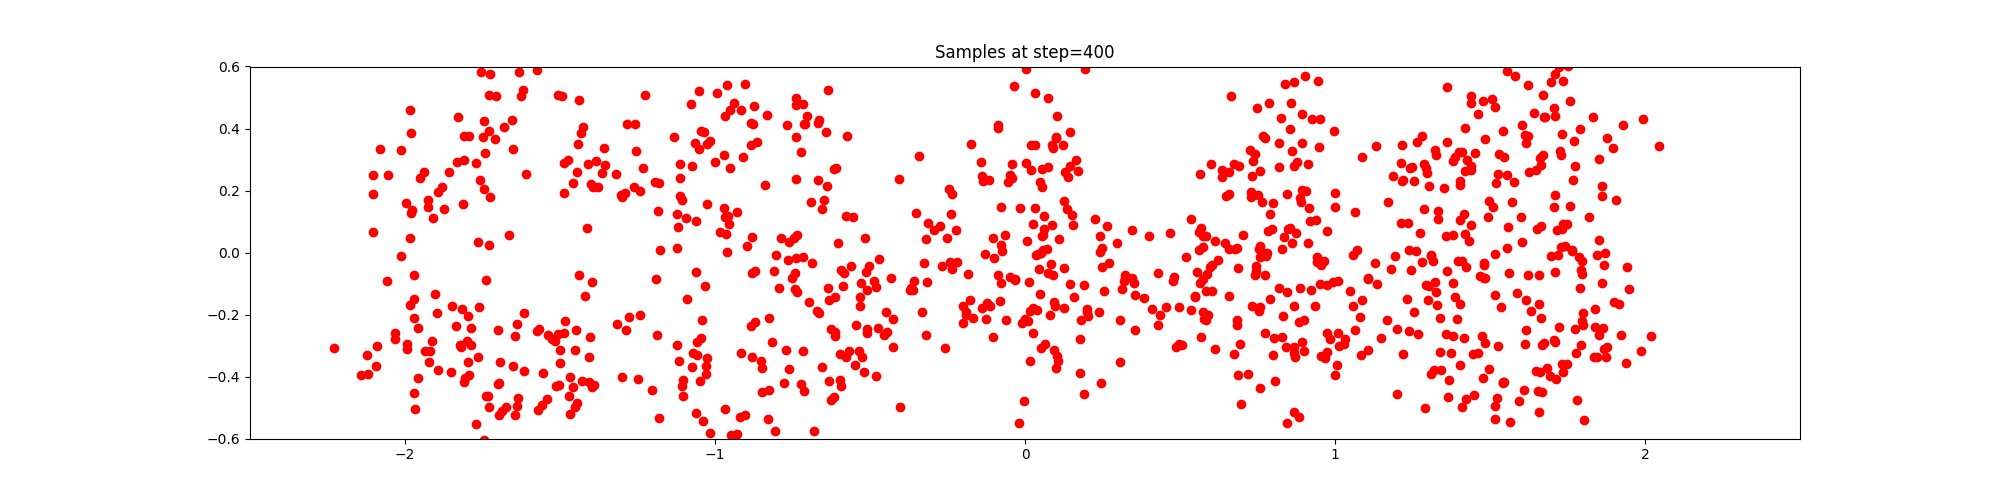
\includegraphics[width=\linewidth]{step_400}
        \caption{Points at time step 400}
    \end{figure}
    \newpage
    \begin{figure}[!h]
        \centering
        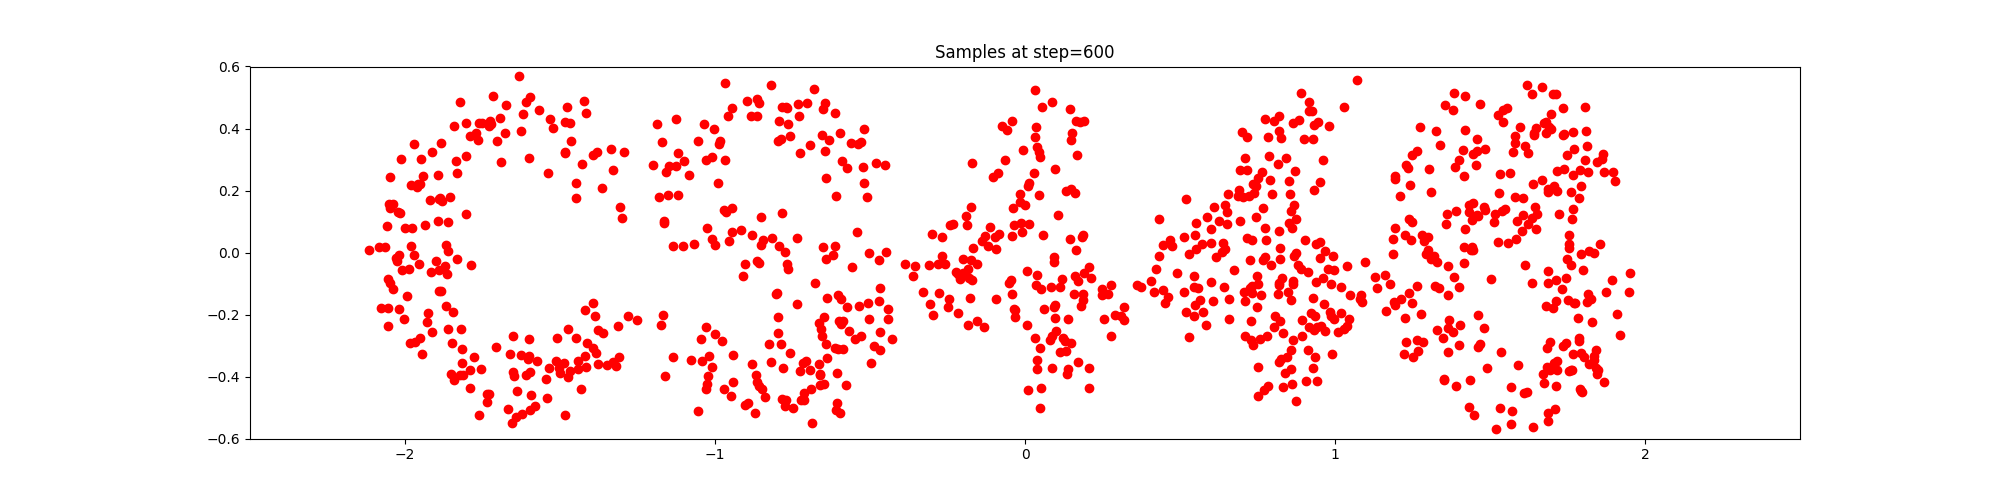
\includegraphics[width=\linewidth]{step_600}
        \caption{Points at time step 600}
    \end{figure}
    \begin{figure}[!h]
        \centering
        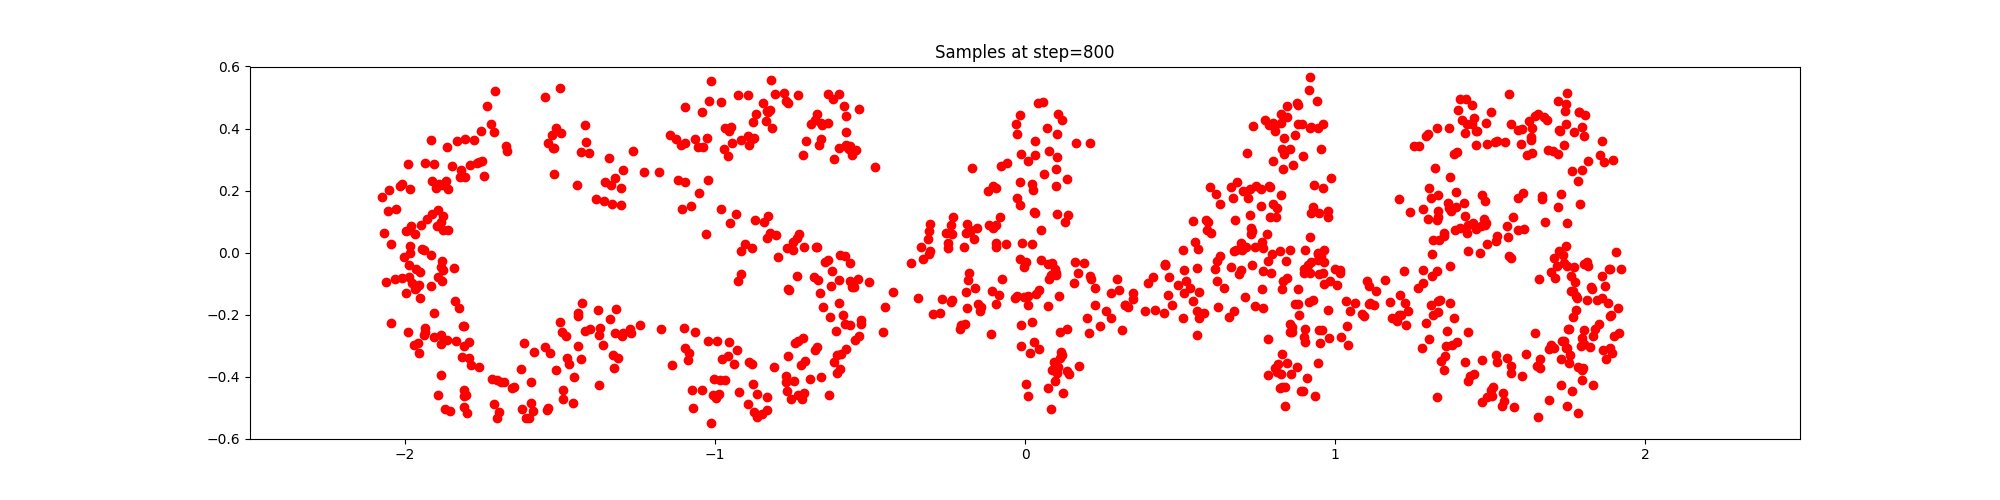
\includegraphics[width=\linewidth]{step_800}
        \caption{Points at time step 800}
    \end{figure}
    \begin{figure}[!h]
        \centering
        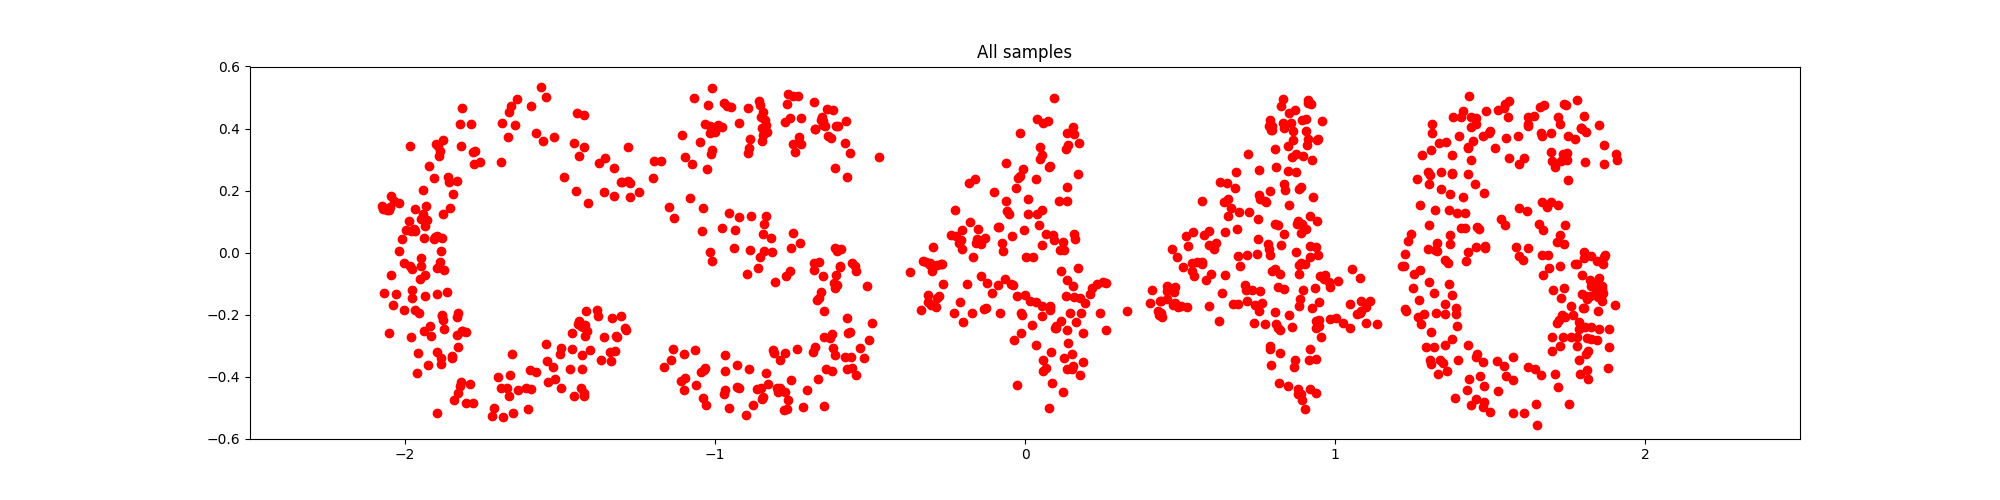
\includegraphics[width=\linewidth]{final}
        \caption{Final sampled points}
    \end{figure}
    \newpage

    \item[(c)] Visualization of the trajectory of langevin dynamics:
    \begin{figure}[h]
        \centering
        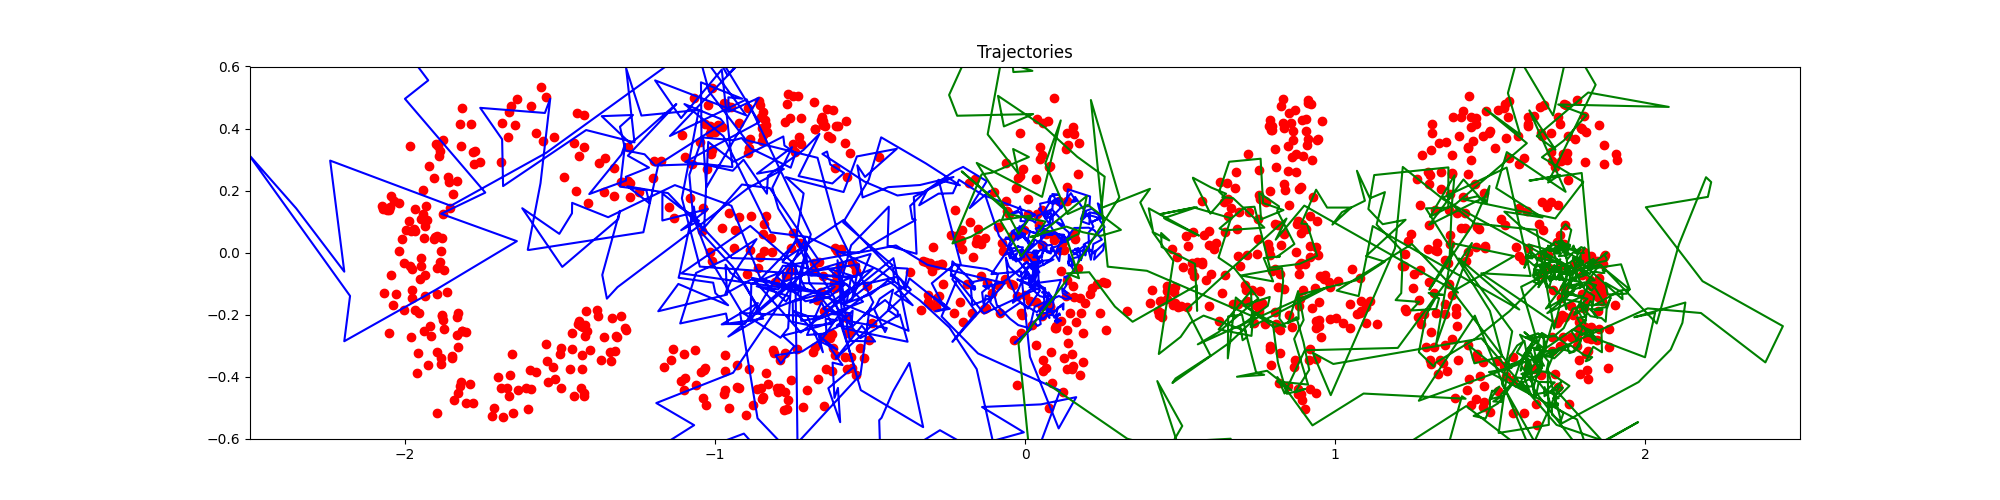
\includegraphics[width=\linewidth]{trajs}
    \end{figure}
    
\end{enumerate}
\end{document}
